\chapter{Preparing Atoms for Interferometry}\label{chap:atom_prep}
\section{Chapter Overview}
This chapter presents the stages of the experiment which prepare an
ensemble of atoms for interferometry, after they are loaded into the
3D \ac{mot}. After being released from the trap, the atoms are cooled
and launched using a moving molasses, as described
in~\SectionRef{sec:optical_molasses}. Following this, a sequence of
optical and microwaves pulses is used to increase the population in
the \(\ket{1,0}\) ground state and end with an ensemble which has a
narrow velocity spread along the Raman axis. A characterisation of
this is given in~\SectionRef{sec:state_prep}.
\par\noindent
Some sections of this chapter refer to parts of the experiment which
have yet to be introduced. Details on the Raman laser and the
velocity-selective Raman pulse can be found
in~\SectionRef{sec:msquared_laser}
and~\SectionRef{subsec:vel_select}, respectively. A
description of the detection scheme, used to measure the population of
atoms in \(\ket{F=1}\) and \(\ket{F=2}\) is presented
in~\SectionRef{sec:atom_detection}.

\section{Cooling in Optical Molasses}\label{sec:optical_molasses}
A low thermal velocity means that the atoms can be interrogated for a
longer time, $2T$, because the atom cloud spreads out more slowly.
This in turn makes the accelerometer more sensitive because the
interferometer phase is proportional to $T^2$. 
Further cooling is therefore required before the most sensitive
interferometer signal can be achieved. Temperatures well below that of
the Doppler limit (\sivalue{146}{\micro\kelvin} for \ac{rb87}) can be
reached using polarisation gradient cooling~\cite{Salomon1990}. In what follows, the principles of
sub-Doppler cooling using polarisation gradients will not be discussed
in detail, but can be found elsewhere~\cite{Dalibard1989,Berg-Sorensent1992}. 

\par\noindent
This section describes the work towards to cooling and launching the
atoms in a moving optical molasses. It starts with a motivation for
launching the atoms in~\SectionRef{subsec:launching}. The following
section discusses the control of the intensity and frequency of the
light during the molasses stage of the experiment. A description of
the techniques needed to cool the atoms in a moving molasses is then
given in~\SectionRef{subsec:moving_molasses}. Finally, this section
concludes in~\SectionRef{subsec:molasses_imaging} with measurements of
both the temperature and trajectory of the atom cloud which were
measured using a ballistic expansion method.


\subsection{Motivation for Launching}\label{subsec:launching}
As previously discussed in~\SectionRef{sec:theory_double_int}, there
are two pairs of counter-propagating beams which can drive Raman
transitions between the two hyperfine ground states. If an atom can be
stimulated by both pairs, then the additional trajectories this
introduces do not interfere, resulting in a reduction in the fringe
visibility. This problem can be avoided by using the fact that the
Raman transition is Doppler-sensitive to ensure that the atoms are
only driven by one pair of beams. Each pair has an opposite Doppler
shift \(\pm \omega_D = \pm \keff.\textbf{v}\) and so their transition
frequencies are separated by \(2\omega_D\). Therefore, the atoms are
launched so that their centre-of-mass velocity along the Raman axis is
large enough to lift the degeneracy of the two Raman transitions. 

%The light used to drive Raman transitions during the exeperiment is launched into the chamber on two orthogonal axes of a \ac{pm} fibre. These are retro-reflected to produce two counter-propagating beams that are orthogonally polarised to the incoming ones. In the absence of \(\pi\)-polarised light, only \((\sigma^+-\sigma^+)\) or \((\sigma^--\sigma^-)\) pairs of polarised beams can drive Raman transitions. If the incoming beams are circularly polarised, then this can occur using counter-propagating pairs of beams which impart momentum \(\pm \hbar \keff\) to an atom. If an atom can be driven by either pair at each interferometer pulse, this results in two interferometer paths, as well as additional trajectories which do not interfere and hence cause a reduction in fringe visibility.
\subsection{Frequency and Power Control}\label{subsec:molasses_control}
A timing diagram illustrating the power and frequency during the
molasses phase is shown in \FigureRef{fig:molasses_timing}.
After the atoms are loaded into the \ac{mot}, they are released by
switching off the quadrupole field. Once this field has decayed away,
the frequency and intensity of the cooling light are ramped
adiabatically~\cite{Molmer1990}. The frequency of the cooling light is ramped to
-25\(\Gamma\) over \sivalue{1.4}{\milli\second}. Since the repump
light is a sideband of the cooling light, the modulation frequency is
simultaneously ramped up to keep this sideband resonant with the
\trans{1}{2} transition. Additionally, the relative detuning of
counter-propagating \ac{mot} beams is varied so that the atoms are
cooled into a moving molasses
(see~\SectionRef{subsec:moving_molasses}). After this, the intensity
of the light is reduced over \sivalue{5}{\milli\second}. The response
of the output \ac{aom} on the \Muquans laser was calibrated so that we
could apply a voltage ramp that gives an approximately linear
intensity ramp.
\begin{figure}[!htbp]
  \centering
  \fontsize{14pt}{14pt}
  \resizebox{0.7\textwidth}{!}{\input{molasses_timing.pdf_tex}}
  \caption[Molasses stage timing diagram]{Timing diagram for the
    molasses stage of the experiment. After a time \(\tau_\text{a} =
    \sivalue{100}{\milli\second}\), the atoms are released from the
    \ac{mot}. The molasses sequence begins \sivalue{3}{\milli\second}
    later, once the magnetic field from the \ac{mot} coils has decayed
    away. First, the frequency of the cooling light is ramped to \(-25
    \Gamma\) over \sivalue{1.4}{\milli\second}. The relative frequencies
    of counter-propagating \ac{mot} beams are detuned so that the atoms
    are cooled in a moving frame, launching them along a parabolic path
    (see~\SectionRef{subsec:moving_molasses}). Next, the intensity of the
    \ac{mot} light is reduced linearly over \sivalue{5}{\milli\second}. To
    measure the temperature, the atoms are left to expand for a duration
    of \(\tau_\text{exp}\) \sivalue{}{\milli\second}, after which they are
  imaged using the camera.}
  \label{fig:molasses_timing}
\end{figure}
\subsection{Launching in a Moving Molasses}\label{subsec:moving_molasses}

The configuration for launching atoms along the Raman axis is shown in
\FigureRef{fig:moving_molasses}. The forward-propagating beams are
blue-detuned by \(+\delta f_l\) and the backward-propagating ones are
red-detuned by \(-\delta f_l\), so that atoms with a velocity along the
beam axis of \(\vec{v} = \delta f_l \lambda\) are resonant with both
beams. The frequency of each beam is ramped from the initial value by
varying the modulation frequency of its \ac{aom}. This ramp occurs
slowly to ensure strong cooling throughout the period of accelerating
the atoms to their final velocity. As there is
no pair of \ac{mot} beams along the axis of the Raman beams, the
\(\vec{x}\) and \(\vec{y}\) \ac{mot} beams, whose axes are nominally
at $\pm45^{\circ}$ to the Raman axis, are used to launch the atoms. By
controlling the power and alignment of each beam, the net velocity on
the atoms will be along the Raman axis. If the detuning of both pairs
of beams is the same, then the velocity along the Raman axis is given
by \(\vec{v_r} = \sqrt{2} \delta f_l \lambda\)~\cite{Ohshima1995}.
\begin{figure}[!htbp]
  \centering
  \def\svgwidth{0.6\textwidth}\input{moving_molasses.pdf_tex}
  %\resizebox{0.6\textwidth}{!}{\input{moving_molasses.pdf_tex}}
  \caption[Beam configuration for a moving molasses]{Beam
    configuration for a moving molasses. When counter-propagating
    beams are detuned from each other, the atoms are cooled into a
    moving frame where the Doppler shift brings both beams to the same
    frequency. Along the vertical
    axis, the beams are detuned by \(\delta f_v\) so that the cloud is
    launched upwards with a velocity \(v_z = \delta f_v \lambda\). In the
    horizontal plane, the \(\vec{x}\) and \(\vec{y}\) beams are detuned by
    \(\delta f_h\) so that the resultant velocity is along the Raman axis
  \(v_r = \sqrt{2}\delta f_h\lambda\). }
  \label{fig:moving_molasses}
\end{figure}
\par\noindent
As well as launching the atoms horizontally, the atoms are launched
vertically so that they can remain closer to the centre of the chamber
after the free fall time $2T$. This keeps them in a region of more
uniform Raman beam intensity where the pulse area is more homogeneous
across the cloud, giving better fringe visibility. This launch is carried out using the \ac{mot} beams that lie along the
vertical \(\vec{z}\) axis. 
%Under an appropriate choice of launch
%velocity, the centre-of-mass trajectory transverse to the Raman beam
%wavefront can be chosen to maximise the interferometer fringe
%visibility. This is presented in further detail
%in~\SectionRef{subsec:launch_contrast}. 
\par\noindent
\subsection{Imaging the Atom Cloud over Time}\label{subsec:molasses_imaging}
Once released from the trap, the atom cloud is free to expand at a
rate due to its
thermal velocity distribution. In addition to this, the centre-of-mass
moves due to its initial velocity and acceleration due to gravity
(and any other external forces).
The temperature of the cloud $T$ was measured by imaging the
distribution of atoms after allowing the cloud to expand in the dark
for a range of expansion times. A typical atom cloud trajectory is
shown in~\FigureRef{fig:molasses_launch}, in which the cloud was imaged
up to \sivalue{76}{\milli\second} after being released from the trap.

\begin{figure}[!htbp]
  \centering
  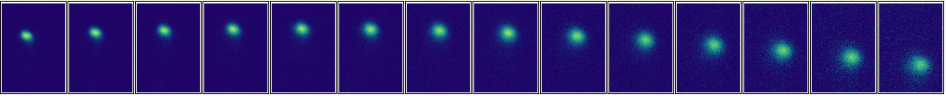
\includegraphics[width=0.8\textwidth]{molasses_launch}
  \caption[Atom cloud position after launching in a moving molasses]{A series of images showing the trajectory of the atom cloud after being cooled in a moving molasses. The first image was taken \sivalue{7}{\milli\second} after initiating the molasses and a subsequent one every \sivalue{5}{\milli\second}. Each image represents a region of interest of dimensions 1150 \(\times\) 1650 pixels that covers the spatial extent of the atom cloud during the launch.}
  \label{fig:molasses_launch}
\end{figure}
\subsubsection{Measuring the Temperature}
In thermal equilibrium, the velocity distribution of the atoms is
described by a Maxwell-Boltzmann distribution. The velocity
component along one direction has the distribution
%\begin{equation}
%    f(v_x,v_y,v_z) = \left(\frac{m}{2\pi k_B }\right)^{3/2}e^{-\frac{m (v`_x^2+v`_y^2+v`_z^2)}{2 k_B T}}
%    \label{eq:mb3D}
%\end{equation}
%where \(v`_i = v_i - \langle v_i \rangle\) is the difference from the
%average velocity. Along a single axis, the velocity distribution is
%obtained by integrating over the other velocity components. For the
%sake of notation, the following discussion uses \(x\) and \(v_x\) as
%labels for position and velocity, but these are interchangeable with
%the equivalent components along the other axes.
%As~\EquationRef{eq:mb3D} is a product of velocity distributions along
%each axis, the velocity distribution along one axis is 
\begin{equation}
  f(v_x) = \left(\frac{m}{2\pi k_B T}\right)^{1/2}e^{-\frac{m (v_x-\langle v_x \rangle) ^2}{2 k_B T}}
  \label{eq:mb1D}
\end{equation}
%Suppose that there are initially \(n_0 (x) \mathrm{d}x\) atoms within
%the region \((x, x+\mathrm{d}x)\), where \(n_0(x) = n(x, t=t_0)\) is
%the initial atomic density along one axis. During ballistic expansion,
%the atoms redistribute themselves according to their velocity. After a
%time \(t\) of free expansion, the position of an atom initially at
%\(x\) is \(x + v_x t\). 
Assuming that the number density is initially a Gaussian, with a peak
number density \(n_0(x_0)\) at the centre-of-mass,
and a mean square radius projected along $x$ of $\sigma_0^2$, the
number density (projected along $x$)
at later times is given by a convolution with~\EquationRef{eq:mb1D}
\begin{equation}
  n(x,t) = \int n_0(x_0) \left(\frac{m}{2\pi k_B}\right)^{1/2} e^{-\frac{m (v_x-\langle v_x \rangle)^2}{2 k_B T}} e^{-\frac{(x+v_x t - x_0)^2}{2\sigma_0^2}} \mathrm{d}v_x
  \label{eq:density_time}
\end{equation}
where \(\sigma_0\) is the \(1/e^2\) initial width of the cloud. As a
convolution of two Gaussians, \EquationRef{eq:density_time} is also a
Gaussian, with a mean-square radius (projected along $x$) given by
\begin{equation}
  \sigma(t)^2 = \sigma_0^2 + \frac{k_B T}{m} t^2
  \label{eq:expansion_width}
\end{equation}
\par\noindent
\FigureRef{fig:molasses_fit_examp} shows a typical density
profile projected along each axis seen by the camera,
as described in~\SectionRef{sec:imaging}. The width along each
axis is estimated using a non-linear least squares fit
to~\EquationRef{eq:density_time}.
\FigureRef{fig:molasses_temperature} shows the measured cloud width
over a range of expansion times. The
initial measurement was made \sivalue{7}{\milli\second} after the end
of the molasses to allow for enough time to re-lock the laser to
\(-0.5\Gamma\) below the \trans{2}{3} transition and align the bias
field to the \(\vec{z}\) axis so that the atoms could be optically
pumped into the \(\ket{2,2}\) state. 
The slopes of these graphs give the temperatures along the horizontal and vertical axes of the
camera as \(T_x = \sivalue{6.38 \pm 0.11}{\micro\kelvin}\) and \(T_y =
\sivalue{6.38 \pm 0.09}{\micro\kelvin}\), respectively.  
\begin{figure}[htpb]
  \centering
  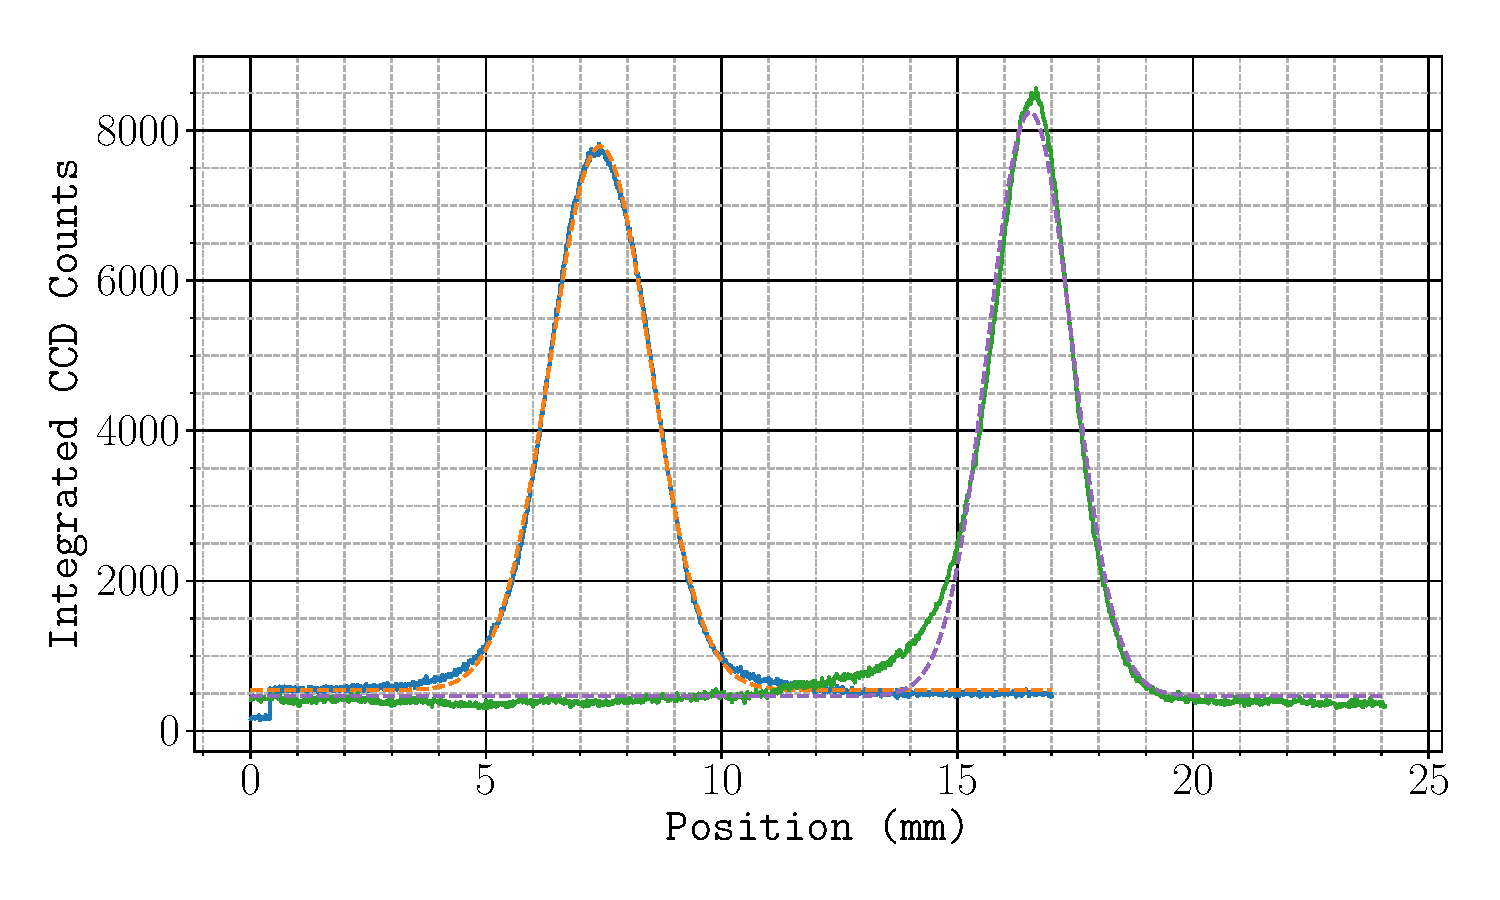
\includegraphics[width=0.8\linewidth]{molasses_fit_examp.pdf}
  \caption[Integrated pixel counts during ballistic expansion.]{Integrated pixel count for a single image during ballistic
    expansion. The dashed lines indicate non-linear least squares fits
  to a Gaussian function.}
  \label{fig:molasses_fit_examp}
\end{figure}
\begin{figure}[!htbp]
  \centering
  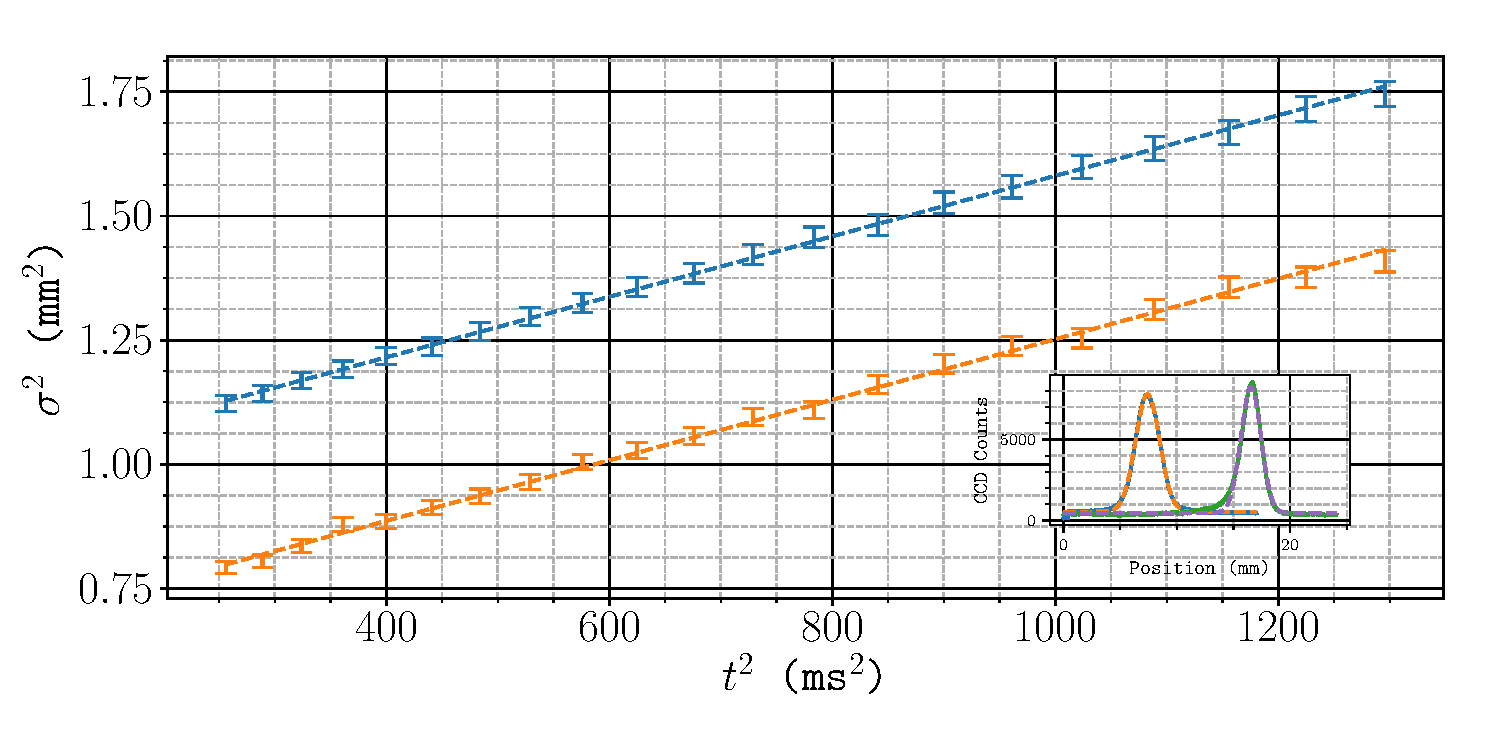
\includegraphics[width=0.8\textwidth]{temperature_launch}
  \caption[Temperature measurement using ballistic expansion]{Mean
    squared cloud radius plotted against the square of the ballistic
    expansion time. After
    molasses, the cloud is left to expand in the dark and in a region of
    close to zero magnetic field. Least-squares fits to the camera
    images give the mean-square radii $\sigma(t)^2$ in the horizontal
    (blue) and vertical (orange) directions. 
    The gradient of these curves gives temperatures \(T_x = \sivalue{6.38 \pm0.11}{\micro\kelvin}\) and \(T_y =
  \sivalue{6.38\pm0.09}{\micro\kelvin}\).}
  \label{fig:molasses_temperature}
\end{figure}

\subsubsection{Measuring the Launch Trajectory}
The same method used to measure the temperature of the cloud can also
be used to measure the position of the centre-of-mass. In this case,
the quantity of interest is \(\langle x(t)\rangle\). Since the cloud
is in free-fall, the trajectory for the centre-of-mass is then given
by the well-known equation-of-motion for a particle moving under
constant acceleration
\begin{equation}
  \langle x(t) \rangle = \langle x(0) \rangle + v_x t + \frac{1}{2} a_x t^2
  \label{eq:position_free}
\end{equation}
where \(v_i\) is the initial velocity along the given axis and \(a_i\)
is the acceleration.
\par\noindent
To launch the atoms vertically, the \((z_+, z_-)\) \acp{aom} were
ramped so that the frequency difference between the light beams was
\(2\times\)\sivalue{320}{\kilo\hertz}. To launch along the Raman
beams, the \(x\) and \(y\) \ac{aom}
frequencies were ramped to give a frequency difference of \(2\times
\sivalue{75}{\kilo\hertz}\) between each pair of horizontal \ac{mot} beams.
\FigureRef{fig:molasses_position} is a plot of the measured
centre-of-mass position along the horizontal and vertical camera axes
over time. A linear least-squares fit
to~\EquationRef{eq:position_free} gives a vertical launch quantities
of \(v_v = \sivalue{25.0\pm0.24}{\centi\meter\per\second}\) and \(a_v
= \sivalue{-9.40\pm0.051}{\metre\per\second\squared}\) and \(v_h =
\sivalue{7.39\pm0.14}{\centi\meter\per\second}\) and \(a_h =
\sivalue{-0.32\pm0.036}{\metre\per\second\squared}\) along the
horizontal axis. 
\begin{figure}[!htbp]
  \centering
  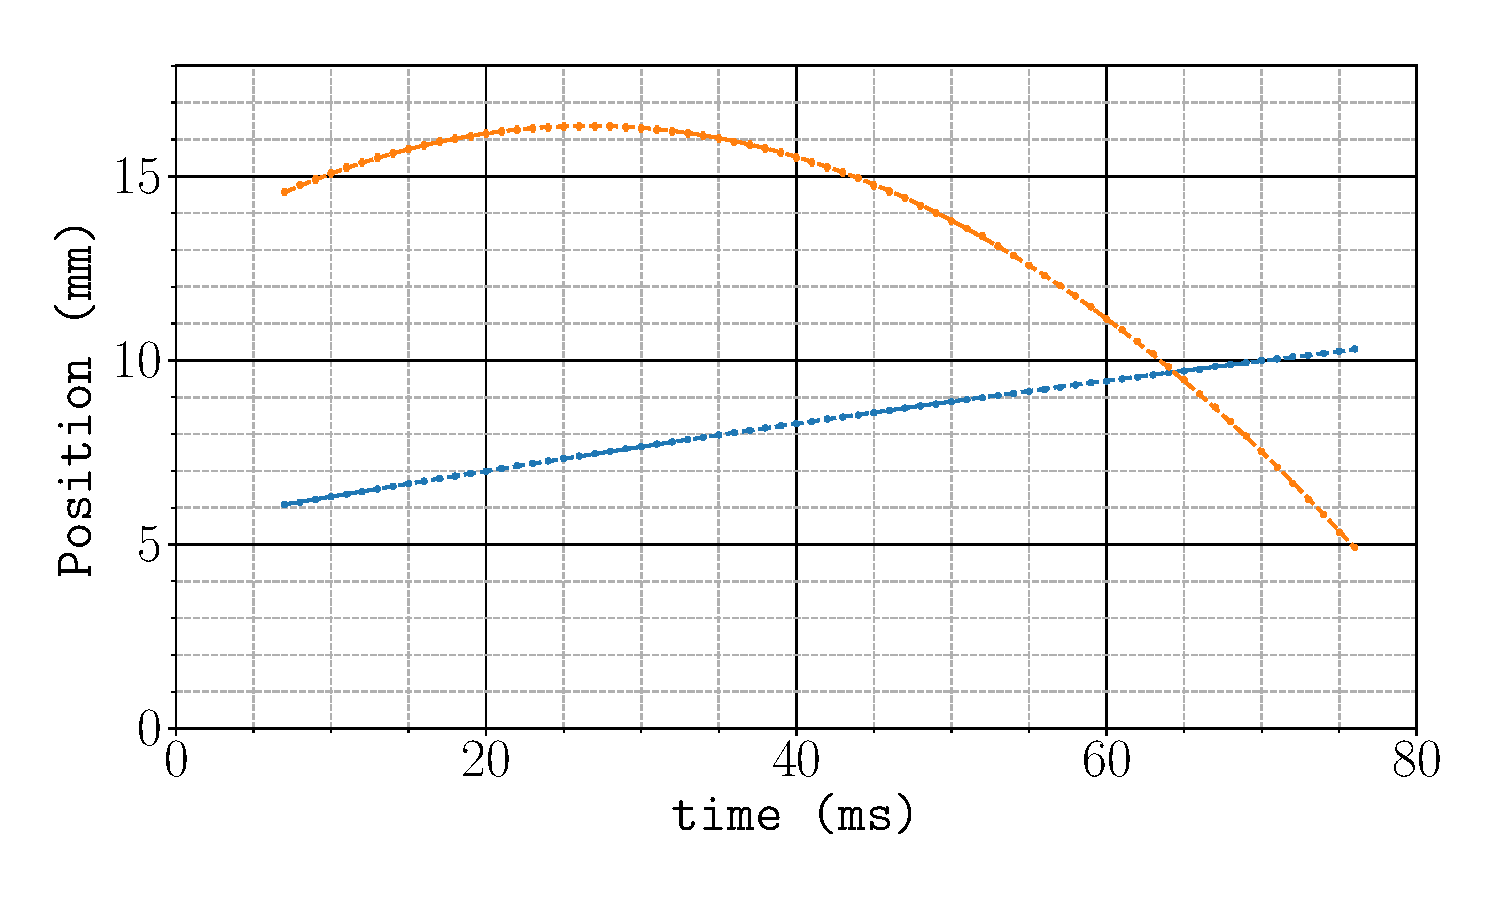
\includegraphics[width=0.8\textwidth]{molasses_position}
  \caption[Atom cloud centre-of-mass over time]{Measured
    centre-of-mass position over time. The horizontal component of the
    position is shown in blue and the vertical in orange. Each
    trajectory is fit to~\EquationRef{eq:position_free} to estimate the
    launch velocity. The best-fit values are \(v_v =
    \sivalue{25.0\pm0.24}{\centi\meter\per\second}\) and \(a_v =
    \sivalue{-9.40\pm0.051}{\metre\per\second\squared}\) along the
    vertical axis and \(v_h =
    \sivalue{7.39\pm0.14}{\centi\meter\per\second}\) and \(a_h =
    \sivalue{-0.31\pm0.036}{\metre\per\second\squared}\) along the
  horizontal.}
  \label{fig:molasses_position}
\end{figure}
\par\noindent
When compared to the expected velocities from the detunings,
\(v^{(l)}_v = \sivalue{24.96}{\centi\metre\per\second}\) and
\(v^{(l)}_h = \sivalue{5.85}{\centi\metre\per\second}\), the measured
horizontal velocity is far greater than expected. This can be
explained by a residual magnetic field, that is not cancelled using
the bias coils. In the presence of a magnetic field, atoms cooled in
an optical molasses are decelerated to a velocity at which the Zeeman
shift is cancelled by the Doppler shift. This velocity-selective
resonance depends on the
orientation of the magnetic field to the polarisation of the light. In
a one-dimensional optical molasses, a resonance occurs at
\(v_\text{res}^{(1)} = - \mu_B g_F B/\hbar k\) when the magnetic field
is aligned with the wavevector of the light \cite{VanderStraten1993}.
When the field is aligned at an arbitrary angle an additional
resonance at \(v_\text{res}^{(2)} = - \mu_B g_F B/2\hbar k\) is
present, due to additional \(\left(\sigma^{\pm}-\pi\right)\)
transitions~\cite{Chang2002,Walhout1992}. A residual field along the Raman axis of
\sivalue{20}{\milli\gauss} would shift the resonance along \(\vec{x}\)
and \(\vec{y}\) by \sivalue{1.09}{\centi\metre\per\second}
corresponding to a velocity of \sivalue{1.54}{\centi\metre\per\second}
along the Raman axis. The magnetic field inside the chamber is
controlled using bias coils and no attempt was made to cancel magnetic
field gradients. It is plausible that a residual field of this
magnitude is a result of a magnetic field gradient. For the moment,
this does not cause a problem as we simply adjust the molasses
detuning to achieve the desired launch velocity. In future, a
precisely known launch velocity may be required for sensing rotations,
and then it will be necessary to return to this issue.

\section{State Preparation}\label{sec:state_prep}
After the atoms have been cooled in an optical molasses, the
population will mostly be distributed across the \(\ket{F=2,m_F}\)
sublevels,
along with a small fraction distributed across the \(\ket{F=1,m_F}\)
sublevels. The Raman transition only couples the \(\ket{1,0}\) and
\(\ket{2,0}\) states, so atoms in the other hyperfine ground states
cannot participate in the interferometer. In fact, since the
individual Zeeman sub-levels are not resolved during detection, these
background atoms result in a loss of fringe visibility.  
\par\noindent
The following section discusses a method of preparing the atoms to
increase the population in the \(\ket{1,0}\) ground state and minimise
the population in all other states. An overview
of the scheme is given in~\SectionRef{subsec:prep_schemes}. This is
followed by a discussion of the initial steps which optically pump
atoms into the \(\ket{1,0}\) state
in~\SectionRef{subsec:optical_pumping}. A description of the microwave
pulse used to drive atoms into the \(\ket{F=2}\) level is given
in~\SectionRef{subsec:microwaves}. This section concludes with the
method used to blow away the atoms which do not contribute to the
interferometer in~\SectionRef{subsec:blow_away}. A key step which has
been omitted is the velocity-selective Raman pulse. This is described
in more detail later, in~\SectionRef{subsec:vel_select}.
\subsection{Schemes for Preparation}\label{subsec:prep_schemes}
The scheme used to prepare atoms in the \(\ket{1,0}\) state is the
following:
\begin{enumerate}
    \item Light resonant with the \trans{2}{2} transition pumps all
      the $\ket{F=2}$ atoms
      into the \(\ket{F=1}\) level.
    \item Light resonant with the \trans{1}{0} transition drives (\(\sigma^{\pm}\)) transitions to pump atoms into the \(\ket{1,0}\) dark state
    \item A microwave $\pi$-pulse transfers those atoms to \(\ket{2,0}\)
    \item A long Raman $\pi$-pulse selects a narrow velocity group of
      atoms in $\ket{2,0}$ and transfers them back to $\ket{1,0}$.
    \item The atoms which remain in \(\ket{F=2}\) are blown away
\end{enumerate}
A diagram of the population of each hyperfine ground state and the
laser frequencies used to drive these transitions is given
in~\FigureRef{fig:state_prep}. With the exception of step 4, the light
is provided by the \Muquans laser using the \ac{mot} collimators
aligned to the vertical \(\vec{z}\) axis. The frequency of the cooling
laser and the repump sideband are set so that the relevant transitions
for steps 1 and 2 are addressed. 
\par\noindent
A timing diagram of the state preparation sequence is shown
in~\FigureRef{fig:state_selection_timing}, which indicates the
duration for which each optical or microwave pulse is applied, as well
as the direction of the applied magnetic field. The field is switched
slowly over \sivalue{2}{\milli\second} (which is omitted from the
diagram) to preserve the spin state of each atom. 
\begin{figure}[!htbp]
    \centering
    %\def\svgwidth{0.8\textwidth}
    \fontsize{32pt}{32pt}
    \resizebox{0.8\textwidth}{!}{\input{state_selection.pdf_tex}}
    \caption[State preparation pulse sequence]{Sequence of optical and
    microwave pulses used to prepare an ensemble of velocity-selected
  atoms in \(\ket{1,0}\). The red arrows indicate optical transitions
to and from \(\ket{F=2}\) and equivalently for the blue arrows and
\(\ket{F=1}\). A residual population is left in the \(\ket{1,\pm 1}\)
states, which contributes a background to the interferometer fringes.}
    \label{fig:state_prep}
\end{figure}
\begin{figure}[!htbp]
    \centering
    %\def\svgwidth{0.5\textwidth}
    \fontsize{14pt}{14pt}
    \resizebox{0.6\textwidth}{!}{\input{state_selection_timing.pdf_tex}}
    \caption[State selection timing schematic]{Timing diagram for state selection sequence. The durations labelled are indicative of the time required to drive the atoms into the desired state at each step. After the \trans{1}{0} pumping, the magnetic field is re-oriented along the Raman axis \(\vec{r}\). The \sivalue{2}{\milli\second} field switching time has been omitted.}
    \label{fig:state_selection_timing}
\end{figure}
\subsection{Optically Pumping the Atoms}\label{subsec:optical_pumping}
\subsubsection{Driving the \trans{2}{2} transition}
After the molasses, the frequency of cooling light is
\sivalue{150}{\mega\hertz} below the \trans{2}{3} transition. This can
off-resonantly excite an atom to the \(\ket{F'=2}\) excited level, but
the small scattering rate means that on average, an atom will need to
scatter many photons before it is pumped into the \(\ket{F=1}\) level.
Therefore, to minimise the heating during this pumping process, the
frequency of the cooling light is shifted to be resonant with the \trans{2}{2}
transition.
\par\noindent
\FigureRef{fig:step1_pumping} shows the population in the two
hyperfine ground states as the duration of the \trans{2}{2} light is
increased. The rate at which atoms are pumped into \(\ket{F=1}\)
increases with the strength of the applied magnetic field. At zero
field, there exists a dark state which is a coherent superposition of
the \(\ket{2,m_F}\) states~\cite{Berkeland2002}. Applying a magnetic
field lifts the degeneracy between the Zeeman sub-levels so that this
dark state is no longer stationary. The evolution rate of this dark
state, and hence pumping rate, increases with an increasing Zeeman
shift. At a field strength of \sivalue{3}{\gauss}, the atoms can be
pumped into \(\ket{F=1}\) in less than \sivalue{5}{\micro\second}.
\begin{figure}[!htbp]
    \centering
    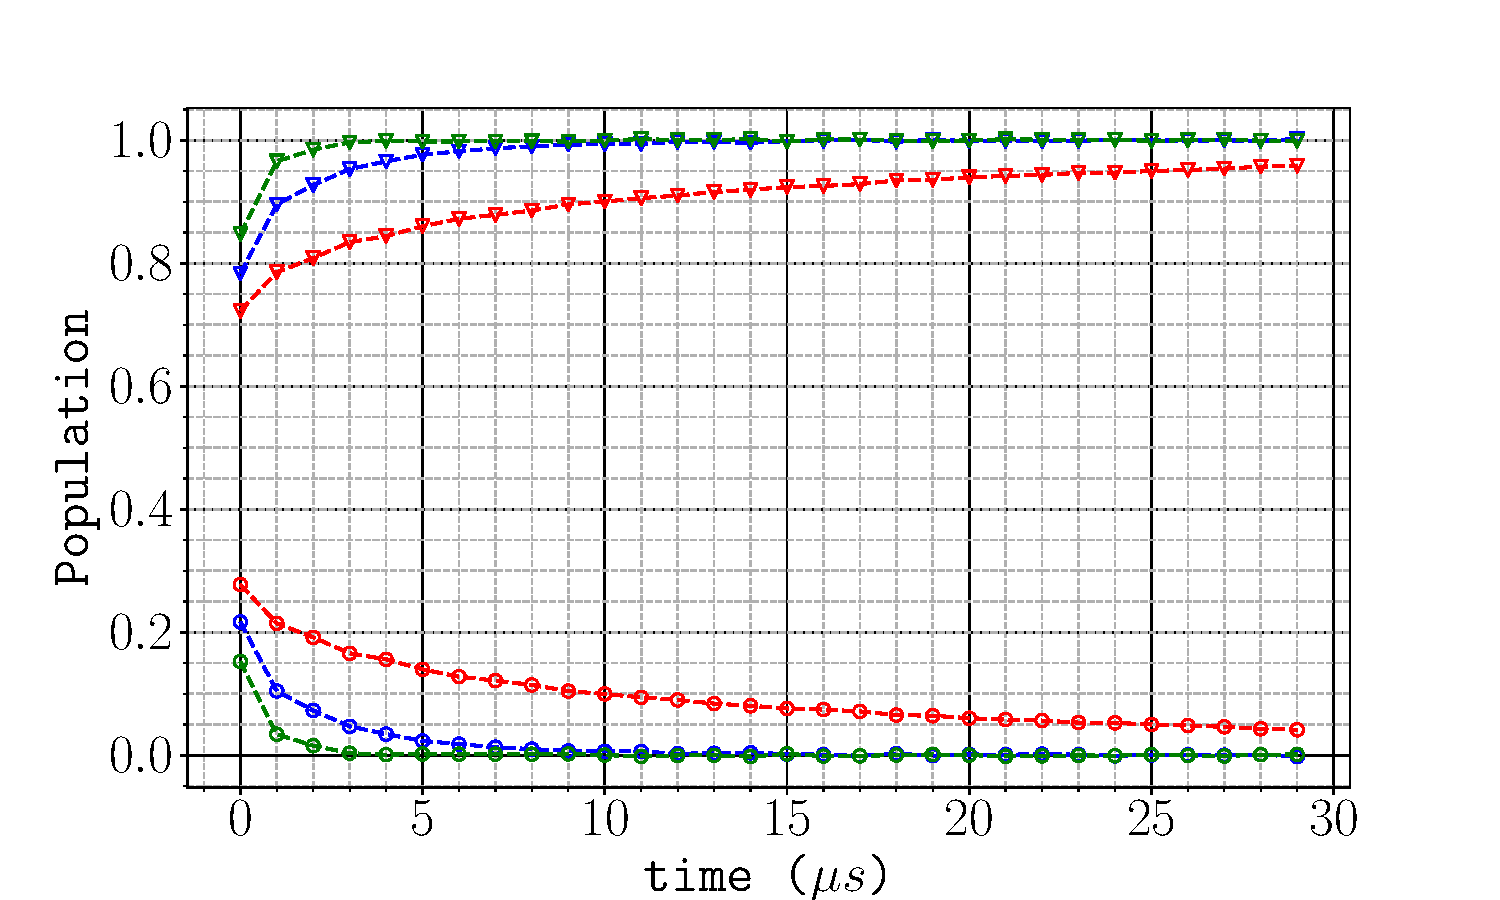
\includegraphics[width=0.7\textwidth]{step1_pumping}
    \caption[Ground state distribution during \trans{2}{2} pumping]{Population across the two hyperfine ground states after \trans{2}{2} pumping under various magnetic field strengths. The $\smalltriangledown$ ($\circ$) markers indicate the population in $\ket{F=2}$ ($\ket{F=1})$. The red, blue and green series correspond to field strengths of \sivalue{-0.16}{\gauss}, \sivalue{1.67}{\gauss}, and \sivalue{3}{\gauss}, respectively.}
    \label{fig:step1_pumping}
\end{figure}
\subsubsection{Driving the \trans{1}{0} transition}
After this first pumping step, the atoms are distributed across the
Zeeman sub-levels in \(\ket{F=1}\). The next pulse of light is used to
increase the population in \(\ket{1,0}\) by driving \trans{1}{0}
transitions. During this time, the \trans{2}{2} light remains on which
helps to prevent atoms from populating the \(\ket{F=2}\) level through
off-resonant \trans{1}{1} excitations. The magnetic field is directed
along $\vec{z}$ so that the circularly-polarised \(\vec{z}\) \ac{mot} beams only
drive \(\sigma^{\pm}\) transitions. This makes the \(\ket{1,0}\) state
a dark state into which all the atoms should be optically pumped. 
\par\noindent
The distribution of atoms across the Zeeman sublevels was measured
using a microwave pulse to drive atoms into the \(\ket{F=2}\) level,
which is described in~\SectionRef{subsec:microwaves}. For each \(\pi\)
microwave transition, the frequency of the microwave field was varied
to find the resonant frequency. The resulting spectra for \(m_F = -1\)
and \(m_F = 0\) are shown in~\FigureRef{fig:step2_microwave_spec},
both with (blue curves) and without (orange curves) applying light to pump into the \(\ket{1,0}\)
state. It can be seen that the $m_F=0$ population is enhanced while
the $m_F=-1$ population is suppressed. From~\FigureRef{fig:step2_mf1}, the first-order
Zeeman shift (\sivalue{1.4}{\MHz\per\gauss}) of the $m_F = -1$ state is \sivalue{-4.435}{\MHz}, which gives a
field strength of \sivalue{3.17}{\gauss}. This is in close agreement
with the value measured from the second-order shift of the 0
\(\rightarrow\) 0 clock transition. The second-order shift of
\sivalue{575.15}{\hert\per\gauss\squared} and the measured shift of
\sivalue{5.6}{\kilo\hertz} correspond to a field strength of
\sivalue{3.12}{\gauss}. 
\begin{figure}[!htbp]
    \centering
    \def\svgwidth{\columnwidth}
    \subfloat[][]{\scalebox{0.5}{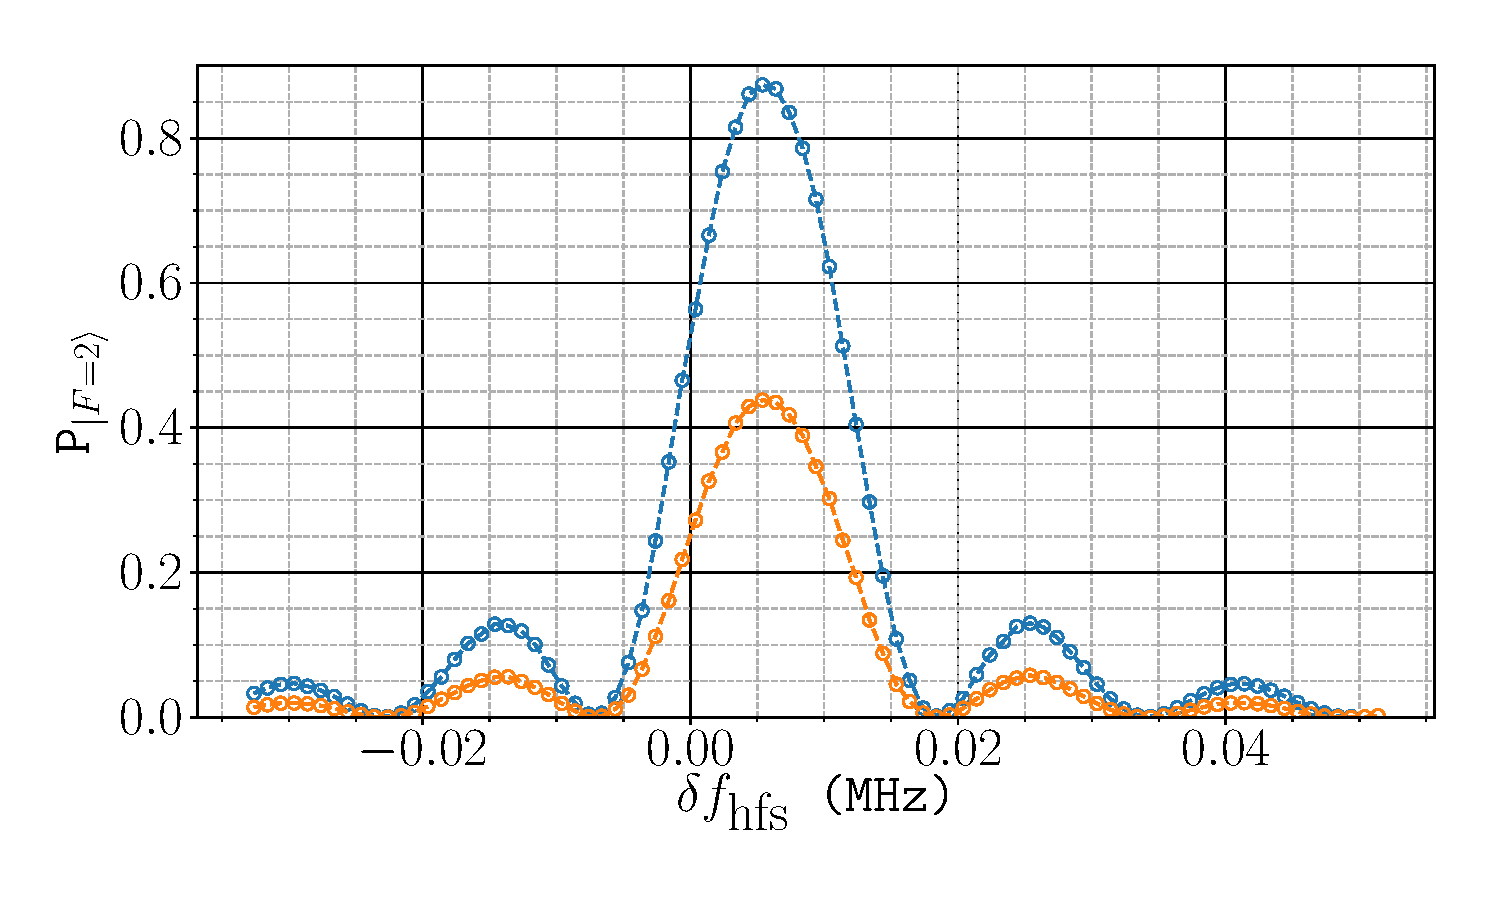
\includegraphics{step2_mf0}}\label{fig:step2_mf0}}\\
    \subfloat[][]{\scalebox{0.5}{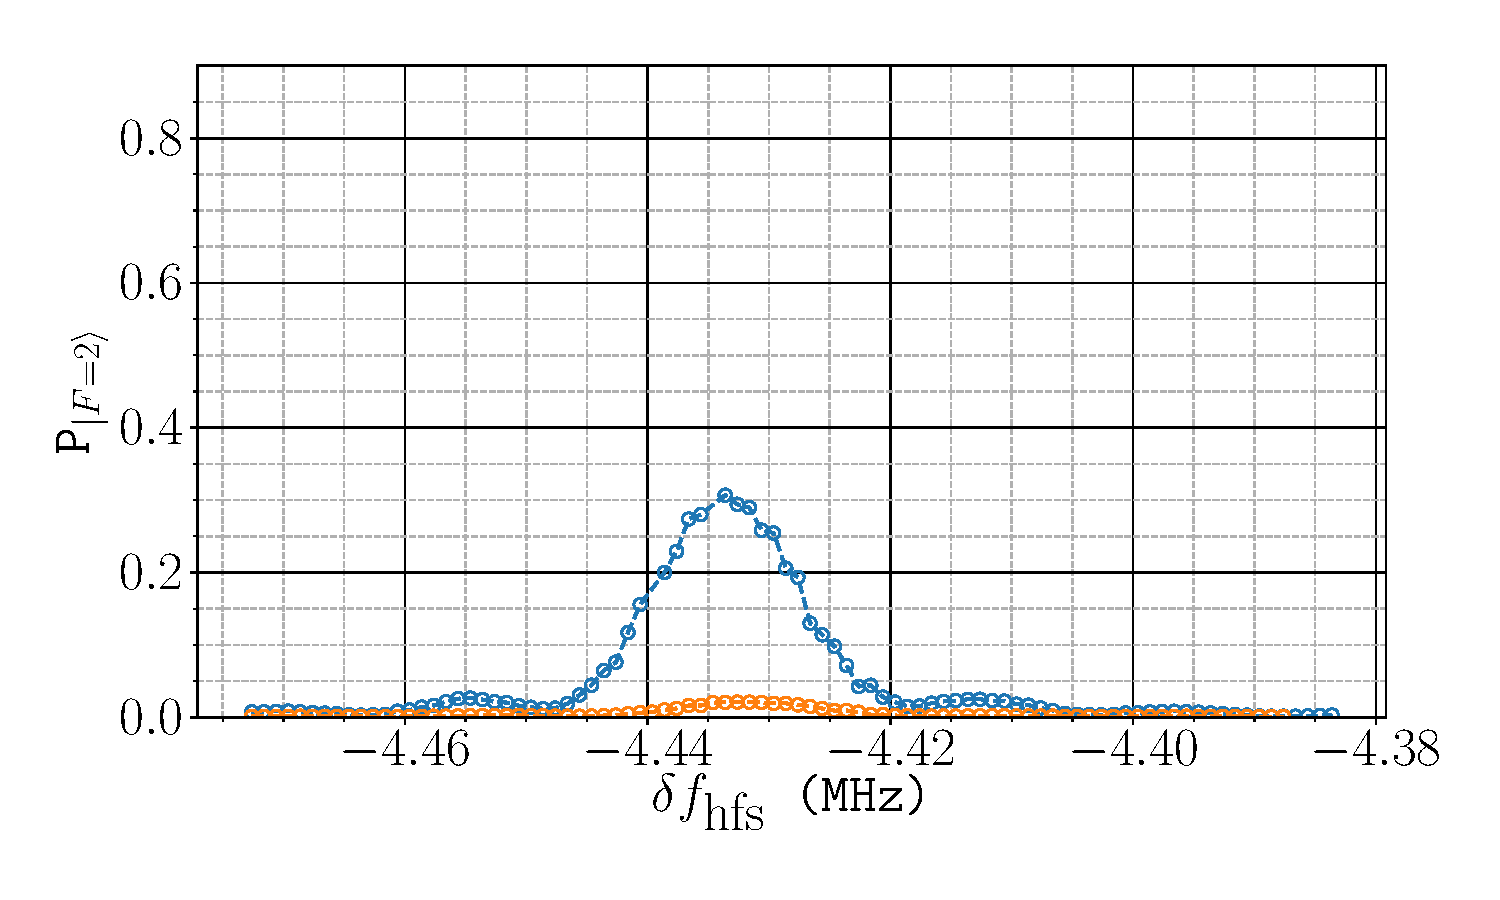
\includegraphics{step2_mf1}}\label{fig:step2_mf1}}
    \caption[\(m_F\) populations before and after \trans{1}{0} pumping]{Population of atoms in (a) \(\ket{1,0}\) and (b) \(\ket{1,-1}\), measured by applying a \sivalue{68}{\micro\second} microwave pulse to drive atoms into the \(\ket{F=2}\) level. The orange and blue points indicate the measured populations with and without \trans{1}{0} pumping. The microwave frequency is plotted as a detuning from the hyperfine splitting frequency \(f_\text{hfs}\).}
    \label{fig:step2_microwave_spec}
\end{figure} 
\par\noindent
A plot of the population in each Zeeman sub-level for increasing
pumping times is given in~\FigureRef{fig:step2_pumping}. In this
instance, the optical pumping does not completely deplete the
population from the \(m_F = \pm 1\) sub-levels. After pumping for
\sivalue{30}{\micro\second}, approximately 5\% of the population
remains in the \(m_F = \pm 1\) sub-levels. The \(\ket{1,0}\) state can
only be excited to \(\ket{F'=0}\) by \(\pi\)-polarised light, which
suggests that the magnetic field is mis-aligned with the \(\vec{z}\)
\ac{mot} beams. If the spherical components $(\sigma^-,\pi,\sigma^+)$
of the dipole operator have values
$(\sqrt{(1-\epsilon^2)/2},\epsilon,
\sqrt{(1-\epsilon^2)/2})$, a value of $\epsilon$ = 0.085 is consistent
with a residual $m_F = \pm 1$ population of 5\%. For circularly
polarised light, a $\pi$-component of this magnitude can be caused by
a mis-alignment of the magnetic field from the $\vec{z}$ axis of
$2.4^\circ$. This is reasonable given that the coils were fixed around
the vacuum chamber without accurately aligning to
the vertical axis of the chamber.

The effect of these background atoms on the measured
interferometer signal is discussed later,
in~\SectionRef{subsec:phase_measurement}.
\begin{figure}[!htbp]
    \centering
    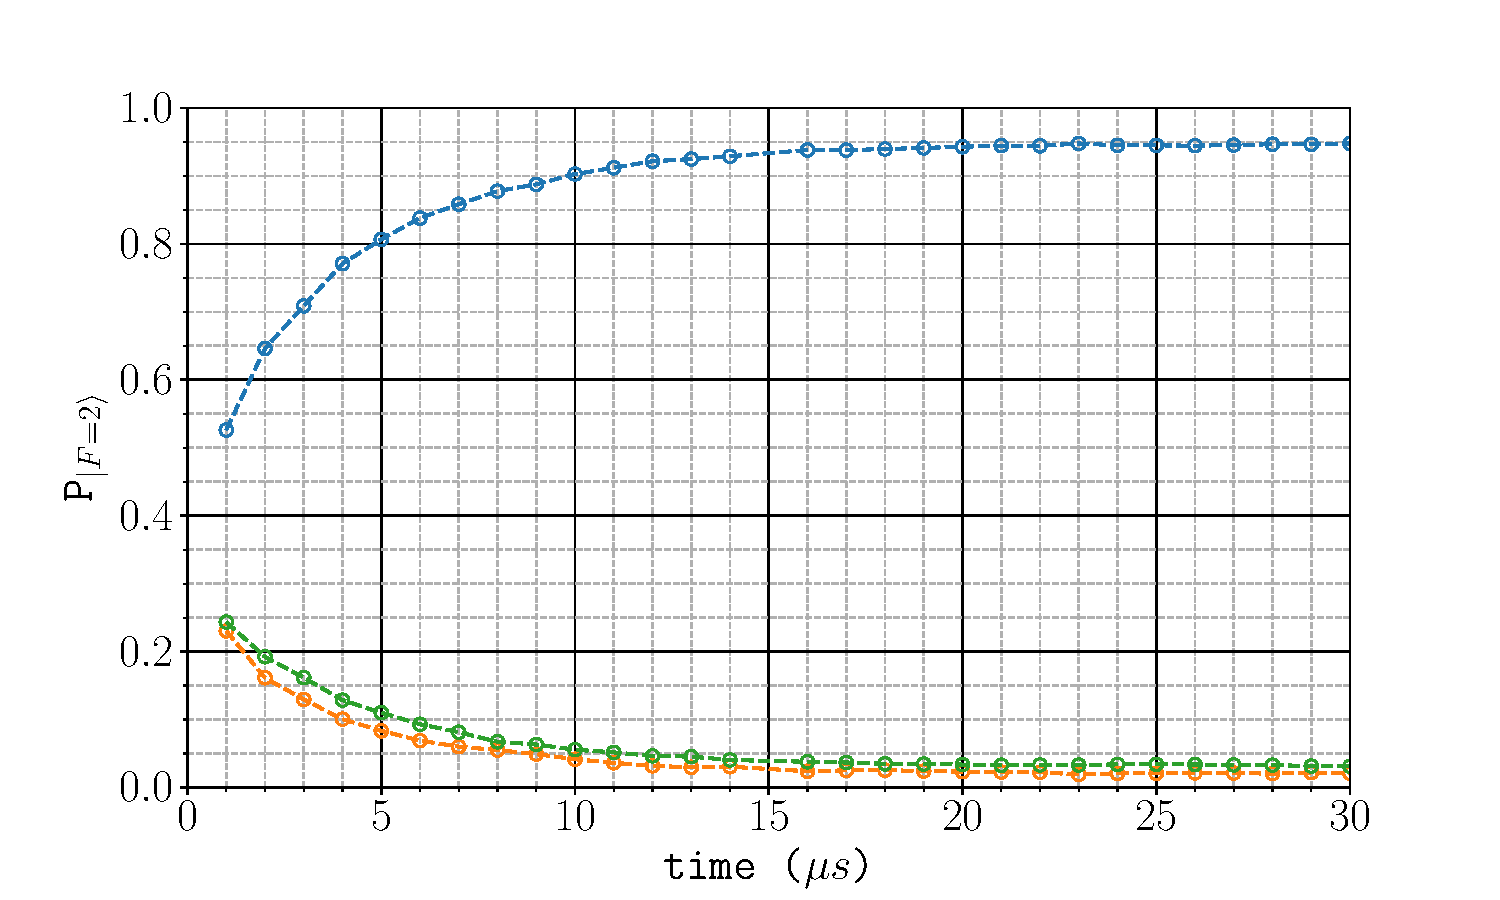
\includegraphics[width=0.8\textwidth]{step2_pumping}
    \caption[\(\ket{1,m_F}\) populations for increasing \trans{1}{0}
    pumping time.]{Population in each Zeeman sub-level as the
    \trans{1}{0} pumping time is increased. The \(m_F = 0, -1, +1\)
  populations are shown in blue, orange and green, respectively. blue
points: with F-1. orange points: without pumping. After \sivalue{30}{\micro\second}, approximately 5\% of the population remains in the \(m_F = \pm 1\) sub-levels.}
    \label{fig:step2_pumping}
\end{figure}
\subsection{The Microwave Transitions}\label{subsec:microwaves}
\subsubsection{Microwave Generation}
A diagram of the microwave setup is shown
in~\FigureRef{fig:microwave_setup}. The microwave radiation is
generated using a \textit{Wind-Freak} synthesiser oscillating at a frequency close to the hyperfine
splitting frequency, \(f_\text{hfs} =
\sivalue{6.83846}{\giga\hertz}\). This is amplified by a
\textit{MiniCircuits MCL ZRON-8G+} amplifier and directed into the
chamber using a \textit{Pasternack PE9859/SF-10} microwave horn, which
produces a linearly-polarised microwave field. The horn was aligned to
the chamber at the position which maximised the population of atoms in
the \(\ket{2,0}\) state. The synthesiser is clocked using a stable
\sivalue{100}{\mega\hertz} signal from the \Muquans{} laser. When the
synthesiser was clocked using its internal \sivalue{27}{\mega\hertz}
reference clock, this produced a noticeable jitter in the output
frequency, which led to a significant shot-to-shot fluctuation in the
\(\ket{2,0}\) population.
\begin{figure}[!htbp]
    \centering
    \resizebox{0.5\textwidth}{!}{\input{microwave_setup.pdf_tex}}
    \caption[Setup for Microwaves]{Schematic diagram of the microwave
    assembly. The frequency close to the hyperfine splitting frequency
  is generated by a \textit{Wind-Freak} synthesiser. A
\sivalue{100}{\mega\hertz} clock signal acts as a stable reference
frequency for the synthesiser. The generated microwave power is
amplified by a low-power \textit{Mini-Circuits}
amplifier, before the microwave horn produces a highly
directional, linearly polarised wave. The output is switched on and
off using one 
digital signal at both the synthesiser and at a bi-directional
microwave switch. The second port of this is terminated to prevent reflections. A USB connection 
to the synthesiser is used to control both its power and frequency.}
    \label{fig:microwave_setup}
\end{figure}
\subsubsection{Pulse Characterisation}
The blue curve in \FigureRef{fig:microwave_spectrum} shows a spectrum obtained by
varying the frequency of the microwave pulse with an applied magnetic field along the $\vec{z}$ axis of
\sivalue{0.67}{\gauss}. This spectrum has a central line due to the
$\Delta m = 0$ transition from $\ket{1,0}$. The peaks on either side
of that are a mix of transitions out of $\ket{1,0}$ and
$\ket{1,\pm1}$. At the far left and right are the peaks from the
$\Delta m = 0$ transitions out of $\pm 1$. The seven transitions that
make up these five peaks are illustrated in
\FigureRef{fig:mw_spectrum_trans}. The orange curve
in~\FigureRef{fig:microwave_spectrum} shows 
that the population in \(\ket{1,m_F=\pm 1}\) is very small after
the \trans{1}{0} pumping step is applied. The linewidth of the
microwave transition is much narrower than the Zeeman splitting, so
only the clock transition is driven when a pulse with a frequency
close to \(f_\text{hfs}\) is applied. 
\par\noindent
\FigureRef{fig:mw_rabi} shows a measurement of the population in the
\(\ket{F=2}\) level for increasing durations of the applied
microwave pulse. Rabi oscillations between the \(\ket{1,0}\) and
\(\ket{2,0}\) states are clearly present. The loss of coherence
between the states can be explained by an inhomogeneous driving field.
Once inside the chamber, the microwaves reflect and scatter off the
interior surfaces which results in a spatially-dependent Rabi
frequency. The data is fit to an exponentially damped Rabi oscillation
given by
\begin{equation}
  \text{P}_{\ket{F=2}} = e^{-\gamma t} \sin(\Omega t)^2
  \label{eq:damped_rabi}
\end{equation}
and gives a characteristic time of $\tau = 1/\gamma =$
\sivalue{1016}{\mus}. It is clear that \EquationRef{eq:damped_rabi}
does not exactly described the observed dephasing. This is not
surprising given that there is no reason that an inhomogeneous
microwave field should give an exponential dephasing rate.
Nevertheless, this indicates that the coherence time between the two
$m_F=0$ states is sufficiently long. The Raman pulses have linewidths
on the order of \sivalue{100}{\kHz}, with durations on the order of
\sivalue{10}{\us}. Over this time, the two states remain coherent.
\par\noindent
A further cause of inhomogeneity is a mis-alignment of the microwave
field to the magnetic field. Referring
to~\FigureRef{fig:mw_spectrum_trans}, the
$\ket{1,m}\rightarrow\ket{2,m-1}$
transitions have the same transition frequency as
$\ket{1,m-1}\rightarrow\ket{2,m}$
transitions. These are the transitions labelled $\textbf{(b)}$ and
$\textbf{(d)}$ in~\FigureRef{fig:microwave_spectrum}. 
The fact that $\sigma^{\pm}$ transitions were observed means
that the microwave field was not parallel with the magnetic field.
Initially, around 
\(85\%\) of the $\ket{F=1}$ population was driven into \(\ket{F=2}\) using a
microwave pulse of \sivalue{100}{\micro\second}. After improving the
alignment of the magnetic field during the microwave pulse, this
fraction increased to \(97\%\) - the remaining 3\% being distributed
across the \(m_F = \pm 1\) states. The strength of the $\sigma^{\pm}$
transitions was also reduced, so that a larger fraction of the
$\ket{1,0}$ population is driven into $\ket{2,0}$. 
\begin{figure}[!htbp]
    \centering
    \def\svgwidth{\columnwidth}
    \fontsize{14pt}{14pt}
    \subfloat[][]{\scalebox{0.5}{\input{microwave_spectrum.pdf_tex}}\label{fig:microwave_spectrum}}
    \subfloat[][]{\scalebox{0.5}{\raisebox{4ex}{\input{microwave_transitions.pdf_tex}}}\label{fig:mw_spectrum_trans}}
    \caption[Microwave transition spectrum]{\textbf{(a)} shows the
      microwave transition spectrum before (blue) and after (orange)
    \trans{1}{0} pumping. The inset is a magnification around $\delta
    f_\textnormal{hfs}$ showing the $m_F = 0$ \rightarrow $m_F' = 0$
    clock transition. \textbf{(b)} shows the transitions addressed
  as the microwave frequency is varied. Dashed and lines indicate
\(\Delta m = \pm 1\) transitions and solid lines indicate \(\Delta m =
0\). In order of increasing frequency, the transitions in \textbf{(a)} are highlighted in: red, blue, green, orange and purple.} 
    \label{fig:microwave_data}'
\end{figure}
\begin{figure}[!htbp]
    \centering
    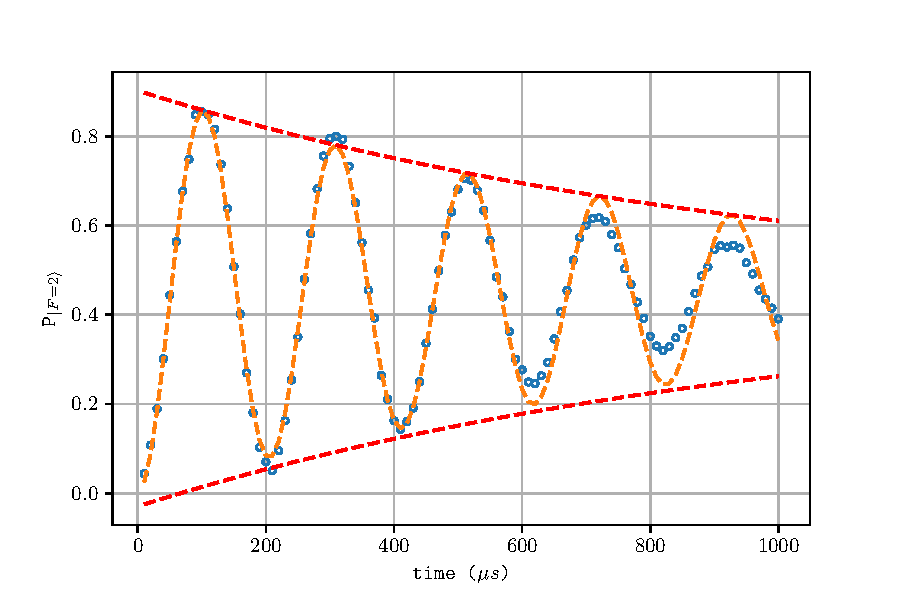
\includegraphics[width=0.7\textwidth]{mw_rabi}
    \caption[Microwave Rabi oscillation between \(\ket{1,0}\) and \(\ket{2,0}\)]{Damped Rabi oscillation between \(\ket{1,0}\) and \(\ket{2,0}\) using a microwave pulse of varying length. At longer pulse times, there is a loss of coherence due to a dephasing between the two states. The red dashed line is an envelope is a fit to a decaying exponential with a characteristic time of \(\tau = \sivalue{1016}{\micro\second}\).}
    \label{fig:mw_rabi}
\end{figure}

\subsection{Blow-Away}\label{subsec:blow_away}
After the atoms populate \(\ket{2,0}\), a velocity-selective Raman
\(\pi\)-pulse is applied to transfer a fraction of those back into
\(\ket{1,0}\)~\cite{Kasevich1991a}. This step is discussed in detail
in~\SectionRef{subsec:vel_select}. The velocity-selective Raman pulse
transfers 4\% the atoms
back to \(\ket{1,0}\). The atoms remaining in $\ket{F=2}$ need to be removed, otherwise
they contribute a large background signal to the interferometer
fringes. \par\noindent
The final pulse during the state preparation sequence is used to push
these non-contributing atoms out of the interferometer region. A
single \ac{mot} beam is used so that there is a net momentum transfer
to the atoms as they absorb light and fluoresce. The frequency of this
blow-away beam is detuned from the \trans{2}{3} transition by
\sivalue{-3}{\mega\hertz}, which is the same frequency used for
detection (see~\SectionRef{sec:atom_detection}). A pulse of
\sivalue{50}{\micro\second} is enough to remove all atoms in
\(\ket{F=2}\). 

% \subsection{Residual \(m_F = \pm 1\) atoms} \label{subsec:residual_atoms}
% After preparing an ensemble atoms in \(\ket{1,0}\) with a narrow velocity spread and removing those out in \(\ket{F=2}\) which are not resonant with the interferometer pulses, there is still a fraction of atoms in \(\ket{1,\pm 1}\) which will be detected and contribute to a background signal. It is worth highlighting how fluctuations in this background affects the sensitivity of the interferometer to accelerations. Since they are not driven by the Raman transition, they remain in \(\ket{F=1}\). If the number of atoms detected in \(\ket{F=1}\) has a contribution from background atoms, i.e \(N_1 = N_\text{bg}+N_1^{(\phi)}\), then the probability of detecting an atom in \(\ket{F=1}\) is given by
% \begin{equation}
%     P_{\ket{F=1}} = P_0 + \frac{C}{2}\sin{\Delta \phi}^2
% \end{equation}
% where \(P_0 = N_\text{bg}/\left(N_1+N_2\right)\) is the proportion of background atoms out of the total number of atoms.

\section{Conclusion}
This chapter has presented the stages of the experiment which are used
to prepare an ensemble of atoms for interferometry. This requires
cooling the atoms to limit the thermal expansion of the cloud during
interferometry. The atoms are also launched using a moving molasses so
that only one pair of beams is resonant with the Raman transition.
Finally, we then apply a sequence of optical and microwave pulses, to
increase the population of atoms in \(\ket{1,0}\). A
velocity-selective Raman pulse with a narrow linewidth is used to make
the velocity spread along the Raman axis much smaller than the Doppler
width. Aside from some residual population in \(\ket{1,\pm 1}\), the
remaining atoms are removed using a pulse of light close to resonance
with the \trans{2}{3} transition. This results in an ensemble of which
around \(40\%\) of the population contributes to the interferometer
signal, the rest being the atoms that were left in \(\ket{1,\pm1}\).

